%% LyX 2.3.6.1 created this file.  For more info, see http://www.lyx.org/.
%% Do not edit unless you really know what you are doing.
\documentclass[english]{vgtc}
\usepackage[T1]{fontenc}
\usepackage[latin9]{inputenc}
\usepackage{geometry}
\geometry{verbose,tmargin=1in,bmargin=1in,lmargin=1in,rmargin=1in}
\usepackage{graphicx}
\usepackage{booktabs}

\makeatletter
%%%%%%%%%%%%%%%%%%%%%%%%%%%%%% Textclass specific LaTeX commands.
\usepackage{mathptmx}
\usepackage{times}

%%%%%%%%%%%%%%%%%%%%%%%%%%%%%% User specified LaTeX commands.
%% Supported class options:

%\documentclass{vgtc}                          % final (conference style)
%\documentclass[review]{vgtc}                 % review
%\documentclass[widereview]{vgtc}             % wide-spaced review
%\documentclass[preprint]{vgtc}               % preprint
%\documentclass[electronic]{vgtc}             % electronic version

%% ``review'' and ``widereview'' are for review
%% submission, ``preprint'' is for pre-publication, and the final version
%% doesn't use a specific qualifier. Further, ``electronic'' includes
%% hyperreferences for more convenient online viewing.

%% Please use one of the ``review'' options in combination with the
%% assigned online id (see below) ONLY if your paper uses a double blind
%% review process. Some conferences, like IEEE Vis and InfoVis, have NOT
%% in the past.

%% Figures should be in CMYK or Grey scale format, otherwise, colour 
%% shifting may occur during the printing process.

%% We encourage the use of mathptmx for consistent usage of times font
%% throughout the proceedings. However, if you encounter conflicts
%% with other math-related packages, you may want to disable it.

%% If you are submitting a paper to a conference for review with a double
%% blind reviewing process, please replace the value ``0'' below with your
%% OnlineID. Otherwise, you may safely leave it at ``0''.
\onlineid{0}

%% declare the category of your paper, only shown in review mode
\vgtccategory{Research}

%% allow for this line if you want the electronic option to work properly
%%\vgtcinsertpkg

%% In preprint mode you may define your own headline.
%\preprinttext{To appear in an IEEE VGTC sponsored conference.}


%% This is how authors are specified in the conference style

%% Author and Affiliation (single author).
\author{Brendan Robert\thanks{e-mail: bdvision@colostate.edu}}

\makeatother

\usepackage{babel}

\CCScatlist{
  \CCScatTwelve{Human-centered computing}{Keyboards}{}{};
  \CCScatTwelve{Human-centered computing}{Touch screens}{}{}
}

\abstract{Touchscreen-based computers allow rapid experimentation with novel
keyboard layouts compared to physical keyboards. The goal of this
experiment is to compare a traditional QWERTY keyboard layout with
a newer optimized keyboard layout based on a Metropolis algorihm to
see how users perform differently, and also if adding hints helps
users acclimate to the different keyboards any better.}

\begin{document}
\title{Badvision Keyboard}
\maketitle

\section{Introduction}

Touchscreen users are reported to have much more discomfort and fatigue
with touchscreen keyboards \cite{chaparro13} compared to traditional
physical analogues. However, there are environments where touchscreens
are the most appropriate form factor and therefore there is a need
to aid touchscreen users to reduce errors and improve overall efficiency
where possible. Overall this can lead to an improved touchscreen user
experience. Aside from commercial settings where tablets are frequently
used such as industrial and medical, users with poor vision or who
are inexperienced (children) can benefit from visual typing aids as
these classes of users are more likely to look at the keyboard while
typing. \cite{alhabri19} This keyboard would work in place of any
standard soft keyboard overlay. The difference is whereas some keyboards
today offer suggested words above the keyboard overlay, the Metropolis-based
\textquotedblleft Badvision\textquotedblright{} keyboard will highlight
suggested keys for the user to press next. This applies to general
keyboard input but in this limited application the subject domain
will be focused on natural common English phrases. The predictive
text model will not account for technical or scientific words, nor
will it be trained on patterns of text found in programming languages.
This is described more in the Trials section below. This soft keyboard
would be ideally suited for any kind of on-screen overlay input scenario
on a touchscreen such as an iPad or a Surface laptop. However, there
is potential to optimize for smaller screen sizes but that will not
be considered as part of this study.

\section{Background}

\subsection{Reactive Keyboard}
Predictive keyboard features, aka Predictive Text Generation was researched
as early as 1988 by John Darragh \cite{darragh88}. His PhD dissertation
proposes an early model for auto-correction named \textquotedblleft The
Reactive Keyboard\textquotedblright{} (shown in figure \ref{fig:reactive_keyboard}) which to
a good degree also serves a fair empirical study of the area of predictive
text dating back even further to early work by Dennis Ritchie and
Ken Thompson in the form of the UNIX Predict keyboard utility. The
Reactive Keyboard thesis goes into great length to examine various
implementation choices for modeling a search algorithm for predictions
as well, though modern readers are not as confronted with tradeoffs
to achieve efficiency and responsiveness on modern hardware. With
Witten and James, Darragh continued this work further \cite{darragh90}
to take the Reactive Keyboard to implementation on the Macintosh platform.
The implementation of this is more of a smart text editor application
which provides auto-correction suggestions as the user is typing.
The state of the art at the time required users to ask programs to
scan documents for spelling errors, so having a quick and efficient
auto-suggestion feature was at the time a very novel concept, but
in a practical sense the authors note that users with disabilities
such as cerebral palsy reported they felt predictive typing aids were
strongly beneficial. It is worthy of mention this effect is a major
consideration and inspiration to continue examining input methods
to help the disabled! 

\begin{figure}
  \centering
  \includegraphics[width=0.95\columnwidth]{\string"reactive keyboard\string".png}
  \caption{The Reactive Keyboard}
  \label{fig:reactive_keyboard}
\end{figure}

\subsection{The WiseType Keyboard}
Alhabri et. al propose a tablet keyboard solution named \textquotedblleft WiseType\textquotedblright{}
\cite{alhabri19} which \textquotedblleft combines different visual
representations for grammar and spelling errors, accepted predictions,
and auto-corrections.\textquotedblright{} WiseType (figure \ref{fig:wisetype_keyboard}) provides
a smart delete key which allows the user to go back to the start of
their first mistake, however on-screen feedback is limited to the
area of text entry itself. The keyboard overlay shown offers no visual
feedback on its own except for suggested words that appear over the
keys, like modern keyboard overlays on modern smart phones. Also like
some modern touchscreen keyboards, WiseType also auto-corrects words
in some cases.

\begin{figure}
  \centering
  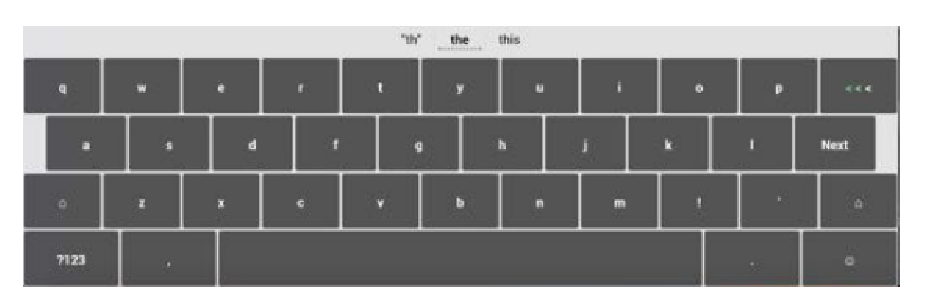
\includegraphics[width=0.95\columnwidth]{WiseType}
  \caption{WiseType Keyboard}
  \label{fig:wisetype_keyboard}
\end{figure}

\subsection{Projection overlay}
Sono and Hasegawa \cite{Sono19} propose projection mapping (figure
\ref{fig:overlay}) onto a physical keyboard as an instructional aid to teach typing.
In the case of this typing tutor approach, the next key expected is
known absolutely and therefore only one key needs to be highlighted
at a time for the user. Their results were reported quantitively in
speed and error, also time to press the first key was measured as
well. They also provided survey results to gauge how confident users
felt about their typing before and after. 

\begin{figure}
  \centering
  \includegraphics[width=0.95\columnwidth]{\string"Overlay Projection\string".png}
  \caption{Sono/Hasegawa Overlay Projection}
  \label{fig:overlay}
\end{figure}

\subsection{The Metropolis Keyboard}
In designing the ideal onscreen keyboard, it became necessary to find
what conclusions have already been reached regarding ideal layouts.
The primary independent variable is to measure user performance against
the presence or absence of typing suggestions, and so the keyboard
layout should also allow greater chance of success. Zhai, Hunter and
Smith designed a keyboard layout (figure \ref{fig:metropolis}) quantitatively using a
Metropolis random walk algorithm to produce a layout capable of 43.1
WPM performance. \cite{Zhai00}

\begin{figure}
  \centering
  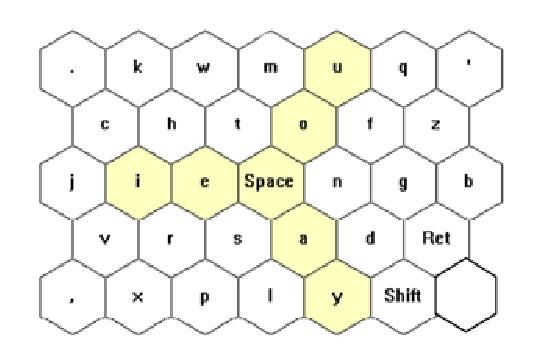
\includegraphics[width=0.95\columnwidth]{Metropolis}
  \caption{Metropolis Keyboard (unweighted layout)}
  \label{fig:metropolis}
\end{figure}

Though promising, this was further improved by Zhai and Smith one
year later \cite{Zhai01} by weighting the alphabetical ordering of
the letters, helping novice users locate keys more quickly, up to
9\% improvement over the previous Metropolis keyboard. The weighted
layout, shown in figure \ref{fig:metropolis_weighted}, is the layout which will be used in the
experiment alongside a traditional QWERTY layout.

\begin{figure}
  \centering
  \includegraphics[width=0.95\columnwidth]{\string"metropolis keyboard weighted\string".png}
  \caption{Metropolis Keyboard weights biased on alphabetical ordering}
  \label{fig:metropolis_weighted}
\end{figure}


\section{Methodology}

\subsection{Subject Selection}

This experiment is hosted on a website, allowing for a geographically-distributed subject pool.  
The only requirement for participants is that they have access to some kind of touchscreen 
tablet device such as an iPad, Surface or Chrome book. Similar studies have roughly a half 
dozen subjects, with trials taking as long  as 45 minutes. To avoid environmental issues 
(see section on extraneous and  confounding variables) the trial duration should be reduced to
10-15 minute intervals, such that participants can take breaks between trial conditions as 
needed.  This should reduce probability of distraction during the test. Also, longer 
tests with no breaks complicate locating willing volunteers so this solves two problems.
With the number of samples per subjects reduced, a data set comparable
to similar studies can be obtained by increasing the desired subject
pool to approximately 20 subjects if possible.

\subsection{Software Test Apparatus}

Again, the software test apparatus is a hosted website. The participant is
identified by a combination of their IP address and any latent tracking
cookies already stored in their browesr.  That way if the user has to leave
or retry the experiment altogether it can be further examined.
When they first arrive, they are presented with a small page of 
instructions explaining the test.

The participant advances from the first screen by providing optional details 
about themselves such their age range, and if they have any physical conditions, injuries
that affect their ability to use computers normally.


Prior to the first trial a more detailed set of instructions is provided
with a visual demonstration of the keyboard in use. The participant is also
reminded that they can take breaks between each of the trials and encouraged
to complete the trial from a quiet, distraction-free environment if possible.
After this they begin the trials.

Starting each trial, the participant is shown a description of the specific
test conditions and prompted to type OK to begin.  Next, a set of text shown at 
the top of the screen and will be asked to type what they read on the screen. 
As they type their response will be shown below the provided text. As correct
letters are typed, the letters in the prompt text are darkened. Incorrect letters
will appear in the typed response but will not advance the progress indication
in the above prompt text.  If they omit one letter and type the next letter proceeding it
then the indicator will act as if they had typed both letters, even though their response
will show they did not actually type it.  The goal is to have a somewhate
fault-tolerant input that does not require the user to correct mistakes so
that they can stay focused on pressing the next keys in sequence, otherwise
measuring typing performance and accounting for user corrections adds
more noise to the data. This fault tolerant behavior is present
for all trials. 

Explored further in the later section on confounding
variables, consistency of physical size of the keyboard layout is
important. For example. a relatively common keyboard such as Logitech K830 
has keys laid out in a 26cm x 10cm arrangement, allowing a compact but usable format. 
In comparison, A Microsoft surface
14\textquotedblright{} laptop has physical view area dimensions larger
than that (28.5cm x 18.5cm), and an iPad Pro has (30.5cm x 22cm).
Ideally the keyboard should vary too much because it could otherwise interfere with
the learned behavior of subjects all of whom are familiar with QWERTY by now.

\subsection{Trials}

The trials run test the same typing test against two independent
variables, Layout and Presence of highlighted key suggestions, each
having two levels. The variations are captured in 4 trials, presented 
to the participant in an order determined by a pre-selected
random sequence that will be assigned to each visitor (4x4 balanced Latin squares).

Ultimately the ideal apparatus being tested is in Trial D, and the
other trials will seek to identify if the independent variables in
that apparatus have any statistical significance in the data observed.

\begin{table}[]
  \centering
  \begin{tabular}{@{}llll@{}}
  \toprule
  Trial & Layout     & Hints & Description \\ \midrule
  0     & QWERTY     & No    & QWERTY    \\
  1     & Metropolis & No    & Metro, aka Zhai-Smith  \\
  2     & QWERTY     & Yes   & QWERTY+Hints  \\
  3     & Metropolis & Yes   & Metro+Hints, aka Badvision   \\ \bottomrule
  \end{tabular}
  \caption{The trials show a combination of two levels for two different independent variables.}
  \label{table:trials}
\end{table}

The four trials are described in Table \ref{table:trials}. For trials
2 and 3, the typing suggestions are offered by highlighting the three
or four most likely keys the user will press next, based on a simple
Markov-chain predictor.  This predictor is  trained against the sample 
set of prompts used. 

The goal is to simulate predictive-like capabilities that
mimic real-world behavior and ensure that one suggestion offered will
always be the correct response. The response of the predictor is a
major factor, it only has to be guaranteed to offer correct predictions
for the typing samples provided so that the user key selection is
reduced to matching from provided samples and the suggestions are
better-than-random, so they are not distracting. 

For example There are some key sequences which will have fewer 
suggestions and might offer only one option, such as if the user types 
\textquotedblleft ZEA\textquotedblright{}
then the only likely next choice is \textquotedblleft L\textquotedblright .
However, the next sequence considered will have more suggestions because
\textquotedblleft EAL\textquotedblright{} might be followed by \textquotedblleft E\textquotedblright{}
or \textquotedblleft A\textquotedblright{} depending on if the user
were typing \textquotedblleft ZEALAND\textquotedblright{} or \textquotedblleft SEALED.\textquotedblright{} 

\subsection{Counfounding and Extraneous Variables}

There are many extraneous variables that cannot be measured or controlled
for this experiment but where possible we can attempt to identify
these and understand their possible effects. Firstly, the subject
pool is a convenience selection, which limits the generalization potential
of the collected data to a wider population. Therefore, in providing
analysis of the results it is important to appropriately frame the
context of the application of this data. Secondly, the subjects will
choose their environment and time for participating in the experiment
and that precludes the ability to offer a distraction-free environment.
The best that can be afforded is a careful wording of the instructions
to ensure the participant is in a quiet distraction-free setting for
the duration of the tests. Also, the user will indicate when they are
ready, so this can help them balance the distractions of their environment 
between trials allowing for breaks. As mentioned earlier,
the test will be designed so trials last no more than 10-15 minutes, hopefully
minimizing the probability of environmental distraction from interfering with
the data. Other than measuring how long they spend on the instruction
pages, there is no reasonable way to measure or control the individual
participants\textquoteright{} environments but hopefully the mitigation
strategies will help.

The confounding variable that affects this experiment
most directly is the level of expertise of the user, specifically
their learned typing proficiency. It is expected that an experience
typist would quickly adapt to the touchscreen and touch-type. Such
users would likely show little or no improvement with the suggested
keys lighting up, because they would not be looking at the keyboard
in the first place. 

We can control this confounding variable to test
the primary independent variable by introducing the second independent
variable of the keyboard layout. This puts the experienced QWERTY
typists on the same level as less-experienced \textquotedblleft hunt-and-peck\textquotedblright{}
typists. Another confounding variable that could affect user performance
is that each user will use their own device which could be any physical
size.

Because of the variety of product dimensions, careful design
will need to be exercised to ensure the physical size of the soft
controls is the similar across devices ahead of time, and the device
used by each participant as well as any detectable settings such as
zoom level should be recorded with the user survey data in case their
device was not accounted for in the apparatus design. Therefore, users will be
requested to use a tablet-sized device to ensure that in landscape
mode it is capable of a near-full dimension of a physical QWERTY keyboard. 

\subsection{Data Collection}

At the beginning of the experiment, a brief survey will be offered
to capture general demographics: 
\begin{itemize}
\item Participant age (provided as ordinal scale of age groups: 5-10, 10-15,
15-20, etc.) 
\item Participant device details (brand/model, open-ended) 
\item Browser user agent string (system-provided) 
\item Where is device relative to user? (In lap, on tabletop, on a stand,
Closed selection)
\item Time and date as well as local user\textquoteright s time zone (system-provided)
\item Physical conditions that impair normal computer use (fatigue, past/present
injuries, visual acuity affects, vertigo, cerebral palsy Closed selection
of options with an \textquotedblleft Other\textquotedblright{} box) 
\item Degree to which they feel it impacts their normal computer use (1-7
scale)
\end{itemize}
For each key stroke in each of the trials, the following will be stored: 
\begin{itemize}
\item Prompt the user is expected to type 
\item Time in milliseconds since the start of the trial when key down was
detected 
\item Time in milliseconds since the start of the trial until key up 
\item The key expected 
\item The key entered (if SKIP that means we detected a skipped key) 
\item If the keystroke was correct (1) or an error (0) 
\end{itemize}
After raw collection is completed for a trial, the information is
then converted into more general information: 
\begin{itemize}
\item Speed, measured in words per minute. Measured as correct keys per second / 5
\item Accuracy, calculated as a percentage of key strokes which were errors or skipped
divided by the length of the original prompt shown. 
\end{itemize}

Both the summary data and the raw data will be retained in case there are additional 
insights of the data that could become useful.

The mean and standard deviation for each trial is then computed.  
Between subjects, the whole series for each of the four trials is compared
with a series of one-way ANOVA comparisons such that the two independent
variables can be considered separately with respect to one of the levels
of the other independent variable at a time.  For example, with hints enabled
(one level of the hint variable), what is the impact, if any, to WPM speed
between the two keyboard layouts.  This is repeated for both WPM and for
accuracy.

\section{Questions/Hypothesis}

With this experiment there are a set of hypothesis and questions to test:

\begin{itemize}
\item For Trial 1 "Zhai/Smith" (metropolis keyboard with no suggestions), will
subjects achieve the WPM speeds above 40 reported in that experiment?
\item With predictive highlighting users should have an easier time learning 
the new keyboard layout, measurable by improved accuracy and WPM speed.
\item Will there be a sufficient number of self-reporting subjects with disabilities,
such that additional benefits to those users can be examined?  This project is not 
specifically studying the effects of this technology on that part of the population 
but having additional options for folks with disabilities can only be a net positive result.
\end{itemize}

\section{Results}
\subsection{Subject summary}
Overall, 36 subjects started the experiment but only 18 completed it.  This is close to the
goal of about 20 subjects, so the incompleted subject data was culled.

Only two subjects reported any kind of impairment that affects typing, so there
was insufficient data to examine those factors.

\begin{figure}
  \centering
  \includegraphics[width=0.95\columnwidth]{subject-age.png}
  \caption{Subjects' ages range from 20 to 80}
  \label{fig:age}
\end{figure}
Subjects' ages range from 20 to 80 shown in figure \ref{fig:age}. Half of subjects (6) are beteen 20 and 24. The rest range equally spread between 40 and 80 years. 
The low sampling value of ages means that finding a correlation between age and typing performance is not
directly possible.

\begin{figure}
  \centering
  \includegraphics[width=0.95\columnwidth]{subject-location.png}
  \caption{Subjects' location}
  \label{fig:location}
\end{figure}
Subjects' location is shown in figure \ref{fig:location}. One third of subjects are located in Ft. Collins.
The rest are from other cities such as Burbank, Des Moines, Newark, and so on.  Other subjects
that did not complete the experiment live as far away as India but are not included in this analysis.

One half of subjects used an iPad, with Windows devices reporting for one third total as well.
Windows users were split 50-50 between Microsoft Surface and other unspecified convertible or hybrid touchscreen
laptops.  Finally, one sixth of subjects use android-based devices, most likely chrome books based on the detected
user agent string sent by their browsers.

Finally, the last random variable examined is the position of the tablet device relative to the user. Close to half
of subjects reported the device sits on the table in front of them.  Another two thirds have the device resting in
their laps.  A smaller number of users are holding the device in-hand (2 total) and finally one subject reports the
tablet is sitting to their side, such as on the arm of a sofa.

Overall, the variety among these random variables adds to the externality validity of this experiment but can arguably
be reasonably considered as threats to internal validity (except for location).  This is discussed later.

\subsection{Speed comparison}
Even though the graph is not normalized to any fixed line, it is clear in the raw data that a correlation exists
between the subject typing speed and the keyboard layout. Furthermore, although subjects using QWERTY type faster,
there is also a much higher degree of variance in the observed standard deviation as well.  On the other side, the
Metropolis keyboard use shows much lower speeds with much lower variance overall as well. Between the Metropolis keyboard
trials with and without hints, the trials with hints very consistently have higher WPM scores with a lower variance as well.

These are analyzed futher in the ANOVA subsection.

\begin{figure}
  \centering
  \includegraphics[width=0.95\columnwidth]{mean-wpm.png}
  \caption{Subject speed in words per minute (WPM). Bubble sizes denote standard deviations.}
  \label{fig:wpm}
\end{figure}

Another analysis is shown in figure \ref{fig:keytime} based on the time between correct key strokes.
For this calculation, incorrect keys are ignored and therefore is a measure only for successful seek
times as an average of all keys during a trial.  For the most part this graph is, as expected, an
inversion of the WPM graph, except it shows the separation between hints and no hints for Metropolis
more clearly: with hints, users were much able to locate the correct keys much more quickly, but not
nearly as quickly as QWERTY in any case.

\begin{figure}
  \centering
  \includegraphics[width=0.95\columnwidth]{time-per-key.png}
  \caption{Subject time per correct key in millisconds. Bubble sizes denote standard deviations.}
  \label{fig:keytime}
\end{figure}

\subsection{Accuracy comparison}

Accuracy analysis allows a different story of the user experience.  This measure is calculated based on the
total number of keys expected in a prompt minus the number of incorrect or skipped keystrokes. This is not
the same number as correct keystrokes (though similar) but rather is the number of non-errored keystrokes.
This number is divided by the total number of expected keystrokes to get a percentage of correct keys in the
range of 0 (completely incorrect) to 1 (zero mistakes.)  One subject of the 18 was observed to have zero mistakes
overall in all trials.  Otherwise, the majority of uses show much lower accuracy for QWERTY (between 65\% and 95\% accuracy)
wheras the range of Metropolis performance is much greater (between 90\% and 98\%.), save one outlier
who had the lowest accuracy overall (~60\%) with a high standard deviation also observed in that same trial.

\begin{figure}
  \centering
  \includegraphics[width=0.95\columnwidth]{accuracy.png}
  \caption{Typing accuracy as a percent of correct keystrokes. Bubble sizes denote standard deviations.}
  \label{fig:accuracy}
\end{figure}

\subsection{ANOVA Analysis}

Between the various trials and measures observed, a series of ANOVA one-way analysis are provided in table \ref{table:anova}.

\begin{table*}[]
  \centering
  \begin{tabular}{c|c|c|c|c|c|c}
  \toprule
  Measure & Constant & Comparison & p-value & f-value & Level 1 mean/std & Level 2 mean/std \\ \midrule
  WPM     & Metro Layout & Hints & ~0.015 & 6.53 & No hints 8.3 +/- 1.4 & Hints 10.0 +/- 2.5 \\
  WPM     & With Hints & Layout & <0.0001 & 52.1 & No hints 8.3 +/- 1.4 & Hints 10.0 +/- 2.5 \\
  WPM     & Metro Layout & Hints & ~0.0152 & 6.53 & No hints 8.3 +/- 1.4 & Hints 10.0 +/- 2.5 \\ \bottomrule
  \end{tabular}
  \caption{ANOVA one-way analysis of various trials.  For each, a single factor is held constant to one level and then the levels of the other variable are compared to each other.}
  \label{table:anova}
\end{table*}

\section{Threats to validity}
\subsection{High external validity, low internal validity}
Given the many combinations of random variables (age, device, position), there is a good argument for the
external validity of this experiment.  However because the orientation of device variances as well as 
the variety of device sizes, it is not as easy to make the same argument for the internal validity at the
same time based on these variables.

However, the apparatus times responses down to the millisecond and therefore data precision is very high.
Also the trials are shuffled in a balanced latin squares order, which clearly removes learning effects
from the results: Consistently the hints are shown to improve perforamnce of Metropolis keyboard use regardless
if the keyboard shows hints the first or second time for the user of that layout. Finally, the subject is
allowed to take breaks between trials and ensure their environment is quiet and distraction-free, which helps
eliminate other random variables not recorded about their surrounding environment. These controls provide
some better internal validity overall.
\subsection{User difficulty during trials}
A small number of users had prompts which required two of the same key in a row to be pressed.
Unfortunately a bug in the apparatus was not anticipated or caught: iPad has a zoom feature activated
by double-tapping on the screen.
There was no significant impact on overall data collection because the prompts were relatively long enough
but this could have limited the maximium potential of users if they were capable of normally typing faster than 50 WPM.

\section{Further exploration}
One possible area of exploration is to measure error not by incorrect 
keystrokes but by the distance between the detected key and the expected key. \cite{Jain11} 
This would allow less of a penalty for keystrokes that were \textquotedblleft fat
finger\textquotedblright{} entries of neighboring keys.

\section{Conclusion}

\bibliographystyle{abbrv}
\bibliography{proposal}

\end{document}
